\documentclass[11pt]{article}
\usepackage[margin=1in]{geometry}
\usepackage{amsmath,amssymb,amsthm,graphicx,booktabs}
\usepackage[hidelinks]{hyperref}
\newcommand{\rtwo}{\sqrt{2}}
\newcommand{\R}{\mathbb{R}}
\newcommand{\err}{e}
\newtheorem{theorem}{Theorem}
\newtheorem{corollary}[theorem]{Corollary}

\title{Quadratic Convergence of Newton's Method\\for the Square Root of Two}
\author{Paper Steward Workshop}
\date{}
\begin{document}
\maketitle
\begin{abstract}
A familiar square-root computation gives a concrete setting in which to distinguish
an exact convergence proof from a finite-precision experiment. Starting at two,
Newton's iteration stays above the positive root, decreases strictly, and converges
quadratically. We derive an exact error identity and compare the iterates with
bisection using reproducible data. The experiment illustrates the analysis while
also exposing the precision limit of floating-point arithmetic.
\end{abstract}
\section{Introduction}\label{sec:introduction}
Computing $\rtwo$ is an elementary problem with a useful lesson about numerical
algorithms: an update rule, a convergence proof, and an implementation are three
different objects. The polynomial $f(x)=x^2-2$ has a unique positive zero, and
both Newton's method and bisection locate it. Their error reduction mechanisms
are very different. Newton uses a derivative to make rapid local progress;
bisection maintains an interval guaranteed to contain a root.

The purpose of this note is to make those mechanisms explicit without relying
on a general convergence theorem. We work in exact real arithmetic for the
analysis, then use binary64 arithmetic for a small illustration. Standard
background on root finding can be found in \cite{burden2015,stoer2002}.
Theorem~\ref{thm:convergence} establishes the main claim, and
Section~\ref{sec:error} explains the quadratic rate.

The example also serves as a compact research-project maintenance exercise.
Its notation, cross-references, bibliography, source code, and derived figures
must stay synchronized. A clean compilation checks document construction;
it does not certify any mathematical assertion.

\section{Newton's iteration}\label{sec:iteration}
At a positive point $x_n$, the tangent line to $f(x)=x^2-2$ has equation
$y=f(x_n)+2x_n(x-x_n)$. Its zero gives
\begin{equation}\label{eq:newton}
x_{n+1}=x_n-\frac{x_n^2-2}{2x_n}
       =\frac12\left(x_n+\frac{2}{x_n}\right),\qquad x_0=2.
\end{equation}
All denominators are nonzero once positivity has been established. Write
$\alpha=\sqrt{2}$ for the positive root. The iteration balances $x_n$ with
$2/x_n$: when the first is above $\alpha$, the second is below it.
Their arithmetic mean nevertheless stays above $\alpha$, as the identity in
the next section shows.

The first two updates are $x_1=3/2$ and $x_2=17/12$. These rational values
already suggest rapid improvement, but a few examples cannot establish
convergence. The proof must show that every subsequent update is defined and
that the only possible limit is the desired root.
% TODO: reconcile notation with shared macros before submission.

\section{Convergence theorem and proof}\label{sec:convergence}
\begin{theorem}\label{thm:convergence}
In exact real arithmetic, the sequence defined by \eqref{eq:newton} satisfies
$x_n>\rtwo$ for every integer $n\geq0$, decreases strictly, and converges to $\rtwo$.
\end{theorem}
\begin{proof}
Let $\alpha=\rtwo$. For any $x>0$, direct algebra using $\alpha^2=2$ gives
\begin{equation}\label{eq:error-identity}
\frac12\left(x+\frac{2}{x}\right)-\alpha
=\frac{x^2-2\alpha x+\alpha^2}{2x}
=\frac{(x-\alpha)^2}{2x}.
\end{equation}
Since $x_0=2>\alpha$, induction shows that each iterate is positive and strictly
above $\alpha$. In particular, the recurrence is defined at every step.
Moreover,
\[x_{n+1}-x_n=\frac{2-x_n^2}{2x_n}<0.\]
Thus the sequence is strictly decreasing and bounded below. It has a limit
$L\geq\alpha>0$. Continuity of $x\mapsto (x+2/x)/2$ on the positive real axis
allows passage to the limit in the recurrence, yielding
$L=(L+2/L)/2$. Consequently $L^2=2$, and positivity forces $L=\alpha$.
\end{proof}
The starting value is part of the statement. A positive start below the root
need not decrease on the first step; a zero start is not defined. More generally,
\eqref{eq:error-identity} puts every positive start other than the root strictly
above the root after one step. We keep $x_0=2$ fixed throughout this note to
avoid mixing this broader observation with the experiment's parameters.

\section{Quadratic error estimate}\label{sec:error}
Define the exact error $\err_n=x_n-\rtwo$. By the theorem it is positive, and
\eqref{eq:error-identity} yields the exact identity
\begin{equation}\label{eq:quadratic}
\err_{n+1}=\frac{\err_n^2}{2x_n}.
\end{equation}
Since $\rtwo<x_n\leq2$, this implies
\[\frac14\err_n^2\leq\err_{n+1}\leq\frac{1}{2\rtwo}\err_n^2.\]
In particular,
\[\lim_{n\to\infty}\frac{\err_{n+1}}{\err_n^2}=\frac{1}{2\rtwo},\]
which is the usual meaning of quadratic convergence with a positive asymptotic
error constant. This ratio statement concerns exact errors, all of which are
nonzero; it is not a claim about errors rounded to zero by a computer.

A quantitative bound follows by setting $q_n=\err_n/(2\rtwo)$.
Then $q_{n+1}\leq q_n^2$, and induction gives
\[\err_n\leq2\rtwo\left(\frac{2-\rtwo}{2\rtwo}\right)^{2^n}.\]
The base is less than one. The double exponent explains why only a few steps
are needed to reach ordinary machine precision. Once rounding errors are of
the same size as the exact truncation error, the recurrence for exact errors
no longer models the computed trajectory accurately. This distinction is
essential when interpreting a plot with a logarithmic axis.

\section{Numerical illustration}\label{sec:numerics}
The script \texttt{experiments/generate\_convergence.py} computes 21 binary64
Newton iterates and 21 bisection midpoints. At index zero the Newton value is
$2$ and the bisection value is the midpoint $1.5$ of $[1,2]$. After each
midpoint evaluation, the sign of $x^2-2$ determines which half interval is
retained. In exact arithmetic the interval length before index $n$ is $2^{-n}$,
so its midpoint error is at most $2^{-n-1}$. Equal indices are not equal-cost
comparisons: Newton requires a division while bisection evaluates a sign.

\begin{table}[ht]
\centering
\begin{tabular}{rrrrr}
\toprule
$n$ & Newton & Newton error & Bisection & Bisection error \\
\midrule
0 & 2.0000000000 & 5.858e-01 & 1.5000000000 & 8.579e-02 \\
1 & 1.5000000000 & 8.579e-02 & 1.2500000000 & 1.642e-01 \\
2 & 1.4166666667 & 2.453e-03 & 1.3750000000 & 3.921e-02 \\
3 & 1.4142156863 & 2.124e-06 & 1.4375000000 & 2.329e-02 \\
4 & 1.4142135624 & 1.595e-12 & 1.4062500000 & 7.964e-03 \\
5 & 1.4142135624 & 1.254e-16 & 1.4218750000 & 7.661e-03 \\
\bottomrule
\end{tabular}

\caption{Initial computed iterates and absolute errors (rounded).}\label{tab:iterates}
\end{table}
\begin{figure}[ht]
\centering
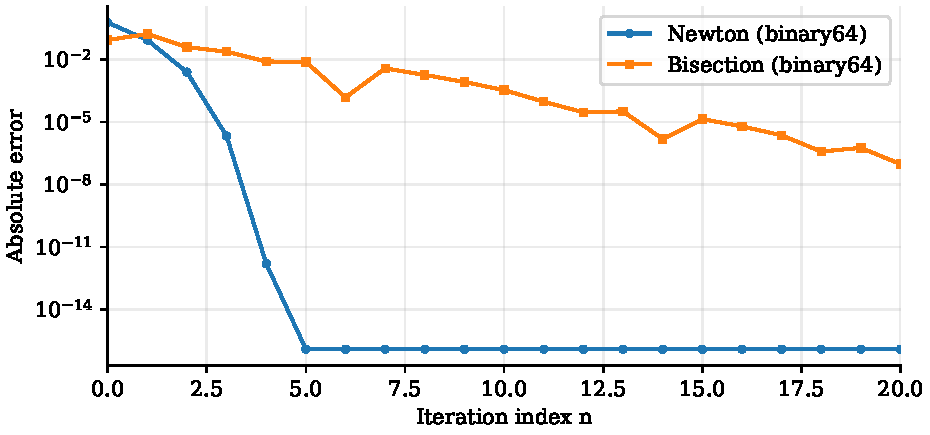
\includegraphics[width=.85\linewidth]{figures/convergence.pdf}
\caption{Computed absolute errors on a logarithmic vertical axis.}
\label{fig:convergence}
\end{figure}

Errors are measured against an 80-digit decimal evaluation of $\rtwo$, using
the exact decimal representation of each computed binary64 value. This avoids
mistaking equality with a rounded binary64 reference for exact accuracy.
For plotting only, errors smaller than $10^{-18}$ are clipped to $10^{-18}$;
the CSV retains the measured errors. The finite reference precision is far
below the scale of this experiment. Newton reaches a rounding plateau near
$10^{-16}$ while bisection continues a slower reduction over these indices.
Neither the observed speed nor the plateau proves the theorem. They illustrate
the exact analysis and the limitations of its floating-point realization.

\bibliographystyle{plain}
\bibliography{references}
\end{document}
